\label{chap:data}

\section{Formal Definition of the Forecasting Task}
\label{sec:data-task}

Let $t\in\{1,\dots,T\}$ index days and let $Y^r_t$ denote the standardised OLR anomaly averaged over region $r\in\{0,\dots,R-1\}$ on day $t$, with $R=50$. For a lead time $L$ (in days), the forecasting task is to estimate $Y^r_{t+L}$ from information available at the issue time $t$:
\begin{equation}
  \hat{Y}^{r}_{t+L} = f_{r}\!\left(\{X^{i}_{t-\ell}: i\in\mathcal{N}_r,\;\ell\in\Lambda\}\right),
  \label{eq:task}
\end{equation}
where $X^i_t$ is the standardised anomaly of node $i$ (Section~\ref{sec:data-matrix}), $\mathcal{N}_r$ is the set of nodes available to the forecaster of region $r$, and $\Lambda$ is the set of input lags. The forecast is \emph{direct}: a separate model maps the state at time $t$ to the value at $t+L$, with no autoregressive roll-out. The primary lead is $L=7$ days, which is the horizon of the research question; $L=1$ day is used as a secondary horizon. The question studied in this thesis is how $\mathcal{N}_r$, the set of source regions available to each forecaster, should be chosen, and whether a validated causal graph is a good basis for that choice.

A forecast is \emph{scored} only if its target day $t+L$ lies in the BSISO active season $\Tseason$ (Section~\ref{sec:data-season}) and in the test period $\Ttest=$ 2013--2022. The inputs may come from any earlier day.

\section{Mathematical Representation of the 300-Node System}
\label{sec:data-matrix}

\subsection{Variables}
The six variables are listed in Table~\ref{tab:variables} with their physical interpretation and role in tropical convection. All are provided as daily anomalies on the native grid.

\begin{table}[htbp]
\centering
\caption{The six Phase~1 variables, their typical physical units before anomaly processing, and their role in tropical intraseasonal convection. The data used here are standardised anomalies and are therefore dimensionless.}
\label{tab:variables}
\footnotesize
\renewcommand{\arraystretch}{1.25}
\begin{tabularx}{\textwidth}{>{\raggedright\arraybackslash}p{1.25cm}>{\raggedright\arraybackslash}p{2.6cm}>{\raggedright\arraybackslash}p{1.45cm}>{\raggedright\arraybackslash}X>{\raggedright\arraybackslash}p{2.6cm}}
\toprule
\textbf{Symbol} & \textbf{Variable} & \textbf{Units} & \textbf{Physical role} & \textbf{Typical time scale} \\
\midrule
SST & Sea surface temperature & K & Surface boundary condition; modulates surface heat and moisture fluxes that sustain convection; responds to cloud shading and wind-driven evaporation & Weeks to months (slow) \\
h850 & Geopotential height at 850\,hPa & m (geopotential metres) & Low-level pressure field; marks the Rossby- and Kelvin-wave response to convective heating and monsoon troughs & Days to weeks \\
u200 & Zonal wind at 200\,hPa & m\,s$^{-1}$ & Upper-tropospheric outflow above convection; large-scale overturning circulation & Days to weeks \\
PW & Precipitable water & kg\,m$^{-2}$ (mm) & Column moisture; strong precursor of deep convection above a critical value~\cite{bretherton2004relationships} & Days \\
u850 & Zonal wind at 850\,hPa & m\,s$^{-1}$ & Low-level monsoon westerlies and moisture convergence; one of the two BSISO index fields~\cite{lee2013realtime} & Days to weeks \\
OLR & Outgoing longwave radiation & W\,m$^{-2}$ & Convection proxy: low OLR indicates cold, high cloud tops~\cite{arkin1987relationship}; the forecast target & Days (fast) \\
\bottomrule
\end{tabularx}
\end{table}

\subsection{Nodes and the state matrix}
A node $i=(r,v)$ is a variable $v\in\mathcal{V}$ averaged over a region $r$. With $R=50$ regions and $|\mathcal{V}|=6$ variables there are
\begin{equation}
  N = R\,|\mathcal{V}| = 50\times 6 = 300
\end{equation}
nodes. Let $\Omega_r$ be the set of grid cells assigned to region $r$ and $\Omega^{\mathrm{ocean}}_r\subseteq\Omega_r$ its ocean cells. The raw regional series is
\begin{equation}
  Z^{(r,v)}_t = \frac{1}{|\Omega^{v}_r|}\sum_{c\in\Omega^{v}_r} A^{v}_{c,t},
  \qquad
  \Omega^{v}_r = \begin{cases}\Omega^{\mathrm{ocean}}_r & v=\mathrm{SST},\\ \Omega_r & \text{otherwise},\end{cases}
  \label{eq:regionmean}
\end{equation}
where $A^v_{c,t}$ is the gridded anomaly of variable $v$ in cell $c$ on day $t$. SST is averaged only over ocean cells because it is undefined over land. Each node is then re-standardised with statistics computed only on the development period:
\begin{equation}
  X^{i}_t = \frac{Z^{i}_t - \mu_i}{\sigma_i},\qquad
  \mu_i = \frac{1}{|\Ttrain|}\sum_{t\in\Ttrain} Z^i_t,\quad
  \sigma_i^2 = \frac{1}{|\Ttrain|}\sum_{t\in\Ttrain}(Z^i_t-\mu_i)^2 .
  \label{eq:standardise}
\end{equation}
The system state on day $t$ is $\mathbf{X}_t=(X^{1}_t,\dots,X^{N}_t)^{\top}\in\R^{N}$, and the full data form the matrix $\mathbf{X}\in\R^{T\times N}$ with $T=16{,}071$ days. Figure~\ref{fig:nodes} shows the structure.

Region means in Eq.~\eqref{eq:regionmean} are unweighted averages of the member cells. On a 2.5\dg\ grid within 30\dg\ of the equator, the cell area varies by at most a factor of $\cos 30\dg\approx 0.87$, so area weighting would change the means only slightly; it is recorded as an implementation choice in Appendix~\ref{app:decisions}.

\begin{figure}[htbp]
\centering
\begin{tikzpicture}[x=0.95cm,y=1cm]
% region blocks
\foreach \r/\lab/\yy in {0/0/0, 1/1/-2.5, 2/2/-5.0, 3/49/-8.0}{
  \node[draw, rounded corners=2pt, minimum width=2.0cm, minimum height=1.25cm, fill=blue!5, font=\footnotesize, align=center] (R\r) at (0,\yy) {Region \lab\\$\Omega_{\lab}$};
  \foreach \v/\nm [count=\k from 0] in {SST,h850,u200,PW,u850,OLR}{
    \pgfmathsetmacro{\py}{\yy+0.9-0.36*\k}
    \ifnum\k=5
      \node[draw, fill=orange!30, minimum width=1.5cm, minimum height=0.3cm, font=\tiny, inner sep=1pt] (n\r\k) at (3.6,\py) {\nm};
    \else
      \node[draw, fill=white, minimum width=1.5cm, minimum height=0.3cm, font=\tiny, inner sep=1pt] (n\r\k) at (3.6,\py) {\nm};
    \fi
    \draw[->, gray] (R\r.east) -- (n\r\k.west);
  }
}
\node at (1.8,-6.6) {\large$\vdots$};
\node[draw, dashed, rounded corners, fit=(n00)(n35), inner sep=4pt] (allnodes) {};
\node[font=\footnotesize, align=left, right=0.4cm of allnodes] (mat) {%
  \textbf{State matrix} $\mathbf{X}\in\mathbb{R}^{T\times N}$\\[2pt]
  $T=16{,}071$ days (1979--2022)\\
  $N=50\times 6=300$ nodes\\[4pt]
  \textbf{Targets:} 50 OLR nodes (shaded)\\
  \textbf{Candidate sources:} all 300 nodes\\
  at lags $\tau=1,\dots,60$ days\\[4pt]
  $300\times 60=18{,}000$ candidates\\ per target};
\node[font=\footnotesize, align=center, above=0.15cm of R0] {Grid cells\\[-2pt](2.5\dg, 30\dg S--30\dg N)};
\end{tikzpicture}
\caption{Schematic of the 300-node representation. Each of the 50 regions contributes six regional-mean variables. The 50 OLR nodes (shaded) are the forecast targets; all 300 nodes are candidate sources at lags of 1--60 days. The diagram is schematic and does not show the real region geometry.}
\label{fig:nodes}
\end{figure}

\subsection{Candidate source--target--lag combinations}
\label{sec:data-candidates}
For one OLR target node $j$, every node $i\in\{1,\dots,300\}$, including $j$ itself, is a candidate source at every lag $\tau\in\{1,\dots,60\}$, which gives
\begin{equation}
  |\mathcal{C}_j| = N\,\taumax = 300\times 60 = 18{,}000
\end{equation}
lagged candidates per target and $50\times 18{,}000 = 900{,}000$ for the 50 OLR targets. If instead every ordered pair of \emph{distinct} nodes were considered with all 300 nodes as targets, the count would be
\begin{equation}
  N(N-1)\,\taumax = 300\times 299\times 60 = 5{,}382{,}000 .
\end{equation}
These numbers count candidate hypotheses before screening, not statistical tests performed: PCMCI's screening stage (Chapter~\ref{chap:pcmci}) removes most candidates after few tests, and the final MCI test is applied only to the survivors. They nonetheless explain why FDR control and an efficient implementation are essential.

\section{Regional Partition}
\label{sec:data-regions}

The native grid has $25\times 144=3{,}600$ cells. Individual cells are noisy and too numerous for a 60-lag analysis, and a single 2.5\dg\ cell has no physical significance. The cells are therefore grouped into 50 regions by $k$-means clustering~\cite{lloyd1982least} applied to the cells' OLR time series over the development period, so that cells whose convection varies together form a region. In practice 46 of the 50 regions are single contiguous areas, and each region contains on average 72 cells. A region adjacency graph is derived from whether any two cells of different regions touch, with longitude wrapping around the date line. The regions are indexed 0--49; this numbering is used in all result figures.

For the resolution check (Section~\ref{sec:val-b4}), each region is split into two sub-regions by $k$-means with $k=2$ applied to its own cells, giving 100 nested regions. Because some sub-regions contain no ocean cells, the 100-region representation has 596 rather than 600 nodes.

Clustering on OLR co-variability and then searching for OLR dependencies between the clusters introduces a mild circularity: regions are, by construction, internally coherent in OLR, and the boundaries between them fall where OLR co-variability drops. The effect is to make between-region OLR links harder rather than easier to detect, but it does mean that the regions are not independent of the target variable. The point is revisited in the threats to validity (Section~\ref{sec:res-validity}). Geographic adjacency, used to define local candidate pools for the forecaster (Section~\ref{sec:moe-pools}), is a separate rule based only on geometry.

\section{Temporal Coverage and Data Provenance}
\label{sec:data-provenance}

Table~\ref{tab:provenance} summarises the data. The fields come from a BSISO monitoring archive in which each variable is stored as a daily anomaly on a common 2.5\dg\ grid covering 30\dg S--30\dg N and all longitudes, from 1 January 1979 to 31 December 2022. The record has 16{,}071 days with no missing days. Each field was anomaly-processed upstream: a daily climatology was removed and the anomalies were normalised separately at each grid cell. A land--sea mask identifies ocean cells for SST.

\begin{table}[htbp]
\centering
\caption{Phase~1 data summary. Items marked [confirm] must be checked against the original archive documentation before submission.}
\label{tab:provenance}
\footnotesize
\renewcommand{\arraystretch}{1.2}
\begin{tabularx}{\textwidth}{>{\raggedright\arraybackslash}p{4.0cm}>{\raggedright\arraybackslash}X}
\toprule
\textbf{Property} & \textbf{Value} \\
\midrule
Archive & Pre-processed BSISO monitoring fields (\texttt{rt\_preprocessed\_archive}); originating reanalysis and OLR products [confirm] \\
Variables & SST, h850, u200, PW, u850, OLR \\
Grid & $2.5\dg\times 2.5\dg$; 25 latitudes (30\dg N to 30\dg S) $\times$ 144 longitudes (0\dg--357.5\dg E) \\
Period & 1979-01-01 to 2022-12-31; 16{,}071 daily values; no missing days \\
Pre-processing upstream & Daily climatology removed and anomalies normalised per grid cell; climatology base period 1979--2014 \\
Auxiliary data & Ocean mask ($25\times 144$, Boolean) \\
Licence & [confirm with archive provider] \\
Development / test split & 1979--2012 / 2013--2022 \\
\bottomrule
\end{tabularx}
\end{table}

\section{Target Construction and Forecast Lead Time}
\label{sec:data-target}

The target of region $r$ at lead $L$ is $Y^{r}_{t+L}=X^{(r,\mathrm{OLR})}_{t+L}$. Two leads are studied:
\begin{itemize}
  \item $L=7$ days, the primary horizon of the research question, at which OLR retains almost no persistence;
  \item $L=1$ day, a secondary horizon at which persistence is very strong and the graph's short-lag links act on the same time scale as the forecast.
\end{itemize}
The input to the forecaster of region $r$ is built from source regions $r'\in\mathcal{C}_r$. For each source region, the six variables are taken at the seven input lags $\Lambda=\{0,1,2,3,5,7,10\}$ days before the issue time, and an ocean-fraction feature is appended, giving a 49-dimensional vector
\begin{equation}
  \mathbf{h}^{r'}_t = \big[\,X^{(r',v)}_{t-\ell}\;:\;v\in\mathcal{V},\;\ell\in\Lambda\,\big]\;\|\;\phi_{r'}\;\in\R^{49},
  \label{eq:features}
\end{equation}
where $\phi_{r'}$ is the ocean fraction of region $r'$ and $\|$ denotes concatenation. The irregular lag set gives dense coverage of the most recent days and sparser coverage further back. The splitter additionally sees a window of the last 10 days of each region's state.

\section{BSISO Season and Activity-Based Target Selection}
\label{sec:data-season}

\subsection{Why an activity-based season}
A fixed calendar window such as May--October treats a year with an early and vigorous BSISO in the same way as a year in which the oscillation is weak until July. Because the graph is meant to describe dependencies that operate when the BSISO is active, the season is defined by the oscillation's own amplitude, with a margin so that onset and decay are included.

\subsection{Reproducing the BSISO index}
The index follows the BSISO1 recipe of Lee \emph{et al.}~\cite{lee2013realtime}, adapted to the available grid:
\begin{enumerate}
  \item OLR and u850 anomalies are taken over 10\dg S--30\dg N, 40\dg--160\dg E. Lee \emph{et al.} use 10\dg S--40\dg N; the data stop at 30\dg N.
  \item The mean of the preceding 120 days is subtracted at each grid point to isolate intraseasonal variability without a non-causal band-pass filter.
  \item Each grid point is weighted by $\sqrt{\cos\varphi}$, where $\varphi$ is latitude, and each field is divided by its domain-mean standard deviation so that OLR and u850 contribute equally.
  \item A combined EOF~\cite{hannachi2007empirical,north1982sampling} is computed on May--October days of the development years only (1979--2012), so that test years never influence the patterns.
  \item The first two principal components are normalised to unit variance over the fit days, and the BSISO amplitude is
  \begin{equation}
    A_t = \sqrt{\mathrm{PC1}_t^2 + \mathrm{PC2}_t^2}.
    \label{eq:amp}
  \end{equation}
\end{enumerate}

\subsection{Season definition}
For each year, the 31-day centred running mean $\bar{A}_t$ of the amplitude is computed inside a search window from 1 April to 30 November. The season starts at the first day of the first run of at least 20 consecutive days with $\bar{A}_t>1$, ends at the last day of the last such run, and is padded by 21 days on each side:
\begin{equation}
  \Tseason_y = \big[\,t^{\mathrm{on}}_y - 21,\; t^{\mathrm{off}}_y + 21\,\big].
  \label{eq:season}
\end{equation}
A year with no qualifying run falls back to 1 May--31 October. The resulting season averages 208 days per year, ranges from 82 to 286 days, and begins between April and July. The development years contain 7{,}153 season days. Figure~\ref{fig:season} in Chapter~\ref{chap:results} shows the amplitude climatology and the season of each year.

The 31-day running mean is centred and therefore uses up to 15 days after a given day. This is acceptable because the season mask decides only \emph{which} target days are scored; it is never an input to a forecast. The consequence is that evaluation is conditioned on the BSISO having been active, which is the intended scope.

\subsection{Target days versus source history}
The season restricts target days only. A source value at lag $\tau$ is read from day $t-\tau$ regardless of whether that day is in the season. For a target on 1 June, a lag-45 source value comes from mid-April. Removing all non-season days before building the lags would delete exactly the precursor information that the analysis is meant to find, and would create artificial discontinuities at the season boundaries. Formally, the PCMCI sample for target node $j$ is
\begin{equation}
  \mathcal{D}_j = \big\{\,(X^j_t,\;\{X^{i}_{t-\tau}\}_{i,\tau})\;:\; t\in\Tseason\cap\Ttrain,\; t-2\taumax\ge 1\,\big\},
  \label{eq:sample}
\end{equation}
where the requirement $t-2\taumax\ge 1$ ensures that the lagged conditioning values of the MCI test (Section~\ref{sec:pcmci-mci}) lie inside the record.

\section{Climatology, Anomalies, Standardisation and Units}
\label{sec:data-anomalies}

\subsection{Why the seasonal cycle must be removed}
Almost every climate variable has a strong annual cycle. Two unrelated series that both peak in boreal summer are strongly correlated at every lag shorter than a few months, purely because of their shared calendar dependence. If the annual cycle were left in the data, PCMCI would find dense, spurious lagged links driven by the calendar, and the forecaster would learn the seasonal cycle rather than intraseasonal dynamics. The standard remedy is to subtract a smoothed daily climatology,
\begin{equation}
  A^{v}_{c,t} = V^{v}_{c,t} - \bar{V}^{v}_{c}\big(d(t)\big),
  \qquad
  \bar{V}^{v}_{c}(d) = \sum_{h=0}^{H} \big[a_{h}\cos(2\pi h d/365.25) + b_{h}\sin(2\pi h d/365.25)\big],
  \label{eq:clim}
\end{equation}
where $V^{v}_{c,t}$ is the raw field, $d(t)$ is the day of year and $\bar{V}$ is a smoothed climatology, here written as the common choice of the mean and first $H$ annual harmonics. The anomalies are then standardised.

\subsection{Implementation in this work}
The fields arrive as anomalies with respect to an upstream daily climatology computed over 1979--2014 and normalised per grid cell. The exact smoothing rule and leap-day treatment of the upstream climatology are those of the archive [confirm]. This work adds two steps: (i) the regional means of Eq.~\eqref{eq:regionmean} are re-standardised with development-period statistics only (Eq.~\eqref{eq:standardise}); and (ii) the BSISO index removes the preceding 120-day mean before the EOF analysis.

The upstream base period overlaps the test period by two years (2013 and 2014). A climatology contains, for each calendar day, an average over 36 years; two of those years being test years means that roughly $2/36\approx 6\%$ of the information in the climatology comes from the test period. The effect on forecast scores is expected to be small, because the climatology is a smooth function of calendar day and all models compared in this thesis share it, but it is a genuine departure from a fully clean split and is listed as a limitation (Section~\ref{sec:res-validity}). Refitting the climatology on 1979--2012 requires reprocessing the gridded archive and is included in future work.

\section{Missing Data and Quality Control}
\label{sec:data-qc}

The archive contains no missing days. Quality control at the regional level consists of (i) checking that every region has at least one ocean cell for SST, which holds at 50 regions but not for 4 of the 100 sub-regions, whose SST nodes are dropped; (ii) checking that each node has a non-zero development-period variance before standardisation; and (iii) confirming that the season mask produces a non-empty season every year. Because there are no gaps, no imputation is performed. A future multi-source dataset (Phase~2) will need an explicit gap and outlier policy.

\section{Lag Construction and Temporal Alignment}
\label{sec:data-lags}

All series share a common daily time axis. For a target day $t$, the candidate value of node $i$ at lag $\tau$ is $X^{i}_{t-\tau}$. Lag $0$ is excluded from graph discovery: a link must point from the past to the present, so its direction follows from time order, and contemporaneous dependence, which cannot be oriented without further assumptions~\cite{runge2020discovering}, is outside scope. For forecasting at lead $L$, the newest usable value of any source is at the issue time $t$, so a source that is a parent of $Y_{t+L}$ at lag $\tau$ can be used directly only if $\tau\ge L$. This forecast-time availability condition is central to interpreting the Stage~C results and is discussed in Section~\ref{sec:moe-availability}.

\section{Development and Holdout Split}
\label{sec:data-split}

\begin{figure}[htbp]
\centering
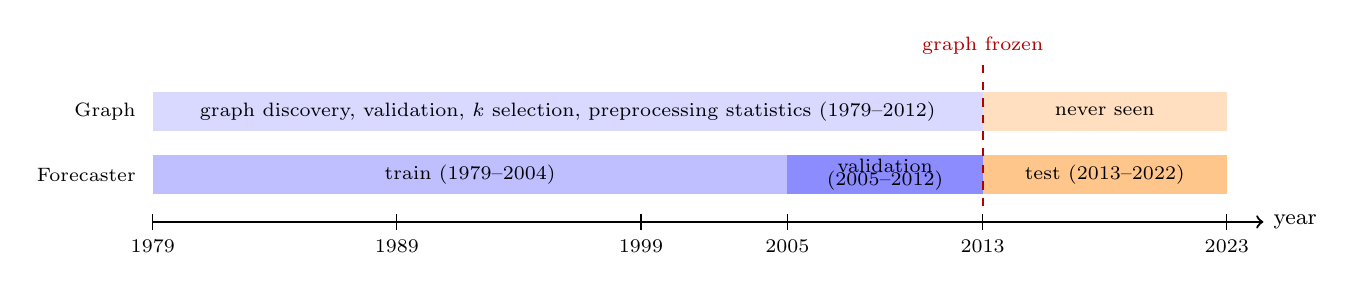
\begin{tikzpicture}[x=0.31cm,y=1cm]
\draw[thick,->] (0,0) -- (45.5,0) node[right,font=\footnotesize]{year};
\foreach \y/\lab in {0/1979, 10/1989, 20/1999, 26/2005, 34/2013, 44/2023}{
  \draw (\y,0.1) -- (\y,-0.1) node[below,font=\scriptsize]{\lab};
}
\fill[blue!25] (0,0.35) rectangle (26,0.85);
\node[font=\scriptsize] at (13,0.6) {train (1979--2004)};
\fill[blue!45] (26,0.35) rectangle (34,0.85);
\node[font=\scriptsize, align=center] at (30,0.6) {validation\\[-3pt](2005--2012)};
\fill[orange!45] (34,0.35) rectangle (44,0.85);
\node[font=\scriptsize] at (39,0.6) {test (2013--2022)};
\fill[blue!15] (0,1.15) rectangle (34,1.65);
\node[font=\scriptsize] at (17,1.4) {graph discovery, validation, $k$ selection, preprocessing statistics (1979--2012)};
\fill[orange!25] (34,1.15) rectangle (44,1.65);
\node[font=\scriptsize] at (39,1.4) {never seen};
\node[font=\scriptsize, anchor=east] at (-0.3,1.4) {Graph};
\node[font=\scriptsize, anchor=east] at (-0.3,0.6) {Forecaster};
\draw[dashed, thick, red!70!black] (34,0.2) -- (34,2.0) node[above,font=\scriptsize]{graph frozen};
\end{tikzpicture}
\caption{Phase~1 time split. Everything that shapes the graph or the forecaster, including the preprocessing statistics, the BSISO EOF patterns, PCMCI, the validation checks and the choice of $k$, uses 1979--2012 only. The graph is frozen before 2013--2022 is used, and test years are used only for scoring.}
\label{fig:timeline}
\end{figure}

Figure~\ref{fig:timeline} shows the split. The development period $\Ttrain$ (1979--2012) is used for graph discovery and for training. Within it, the forecaster uses 1979--2004 for fitting and 2005--2012 for validation, and the top-$k$ check fits on 1979--2004 and scores on 2005--2012 season days. The test period $\Ttest$ (2013--2022) is held out: it provides 1{,}989 season target days for evaluation. A chronological split rather than random cross-validation is used because random folds of autocorrelated series place nearly identical days in training and test sets and overstate skill~\cite{bergmeir2012use}.

\section{Leakage Prevention}
\label{sec:data-leakage}

Leakage occurs when information that would not be available at prediction time influences model construction~\cite{kaufman2012leakage}. Table~\ref{tab:leakage} lists each possible channel and the control applied.

\begin{table}[htbp]
\centering
\caption{Leakage channels and controls in Phase~1.}
\label{tab:leakage}
\footnotesize
\renewcommand{\arraystretch}{1.2}
\begin{tabularx}{\textwidth}{>{\raggedright\arraybackslash}p{4.0cm}>{\raggedright\arraybackslash}X}
\toprule
\textbf{Channel} & \textbf{Control} \\
\midrule
Node standardisation & Means and variances from 1979--2012 only (Eq.~\eqref{eq:standardise}) \\
Regional partition & $k$-means fitted on the development span \\
BSISO EOF patterns & Fitted on May--October days of 1979--2012 only \\
Graph discovery and validation & PCMCI, decoys, lag mask, persistence on 1979--2012 season days only \\
Choice of $k$ & Fit 1979--2004, score 2005--2012 \\
Correlation-prior ranking & Lagged correlations computed on training rows only \\
Forecaster training and early choices & 1979--2004 train, 2005--2012 validation \\
Climatology baseline & Mean of the training targets \\
Upstream anomaly climatology & Base period 1979--2014; two-year overlap acknowledged as a limitation \\
Season mask & Selects scored days only; never an input to a forecast \\
\bottomrule
\end{tabularx}
\end{table}

\section{Unresolved Dataset Decisions}
\label{sec:data-open}

Three dataset decisions remain open and are recorded in the decision log (Appendix~\ref{app:decisions}): (i) confirmation of the originating products and licence of the archive; (ii) refitting of the anomaly climatology on 1979--2012 to remove the overlap with the test years; and (iii) the use of a second, independent reanalysis or OLR product to test whether the graph depends on the data source. None of them affects the internal consistency of the comparisons in this thesis, because every model is evaluated on identical inputs and targets.

\section{Chapter Summary}
\label{sec:data-summary}

This chapter defined the direct seven-day OLR forecasting task, the 300-node representation built from 50 OLR-coherent regions and six variables, the 49-dimensional regional feature vectors, the activity-based BSISO season reproduced from the project's own data, and the development/test split with its leakage controls. The next chapter describes how PCMCI turns the 18{,}000 candidates per target into a sparse lagged graph.
